\chapter{Tool Refactoring Methodology}%
\label{methodology}

\section{Architectural Analysis of Packages within RMT}

To understand the operational dynamics of RMT, it is imperative to analyze the codebase, specifically the various packages. The initial phase of the updating process involves discerning the functionality of different code segments to determine whether to undertake a code refactoring or a comprehensive service rewrite.

\subsection{Intermediary Sevice Packages Analisys}
\label{sub-intermediary-packages}
The intermediary service is systematically divided into four main packages, each comprising functionalities. The first functionality involves the management of refactoring projects. The second pertains to the facilitation of inter-service communication. The third serves as a service discovery mechanism by registering the addresses of all ancillary services to enable seamless subsequent communications. They are illustrated by the package diagram shown in \Cref{fig-package-intermediary}.

\begin{figure}[ht!]
\SetCaptionWidth{\textwidth}
\caption{Intermediary Service Package Diagram}
\label{fig-package-intermediary}
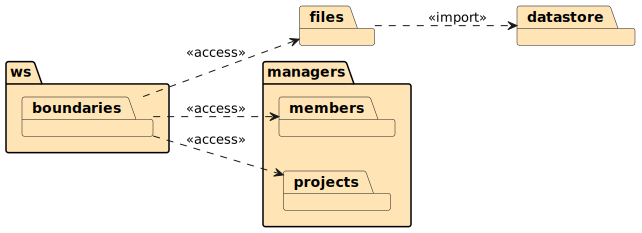
\includegraphics[width =\textwidth, scale=0.2]{Chapter-4/Figures/intermediary-service.png}
\SourceOrNote{Own authorship (2024)}
\end{figure}
\FloatBarrier

The package \texttt{datastore} encompasses all configuration files pertinent to the database pool and the connection configuration.

Package \texttt{ files} contains repository files for database interactions, facilitating queries, insertions, and additional data manipulations.

Within the manager package, the entire outbound logic refers to the refactoring process and the discovery of services, encompassing all related requests for refactoring and generating metrics in the package \texttt{managers.projects} and registering services in the package \texttt{managers.members}.

For handling communication, the \texttt{ws.boundaries} package includes the controller configurations. Within this package, business logic is assigned to the persistence and querying of projects and dispatching requests to other services. Consequently, this package must access the \texttt{managers} and \texttt{files} packages.

\subsection{Detection Service Package Analisys}

The detection service is arranged into six main packages, the core functionalities of which are periodically communicated with the intermediary service to ensure registration with the service discovery mechanism. Moreover, interfaces have been developed to analyze the source code for potential refactoring candidates, and interfaces have been designed to execute refactoring on projects identified as containing such candidates. The package diagram displayed in \Cref{fig-package-detection} illustrates them.
\begin{figure}[ht!]
\SetCaptionWidth{\textwidth}
\caption{Detection Service Package Diagram}
\label{fig-package-detection}
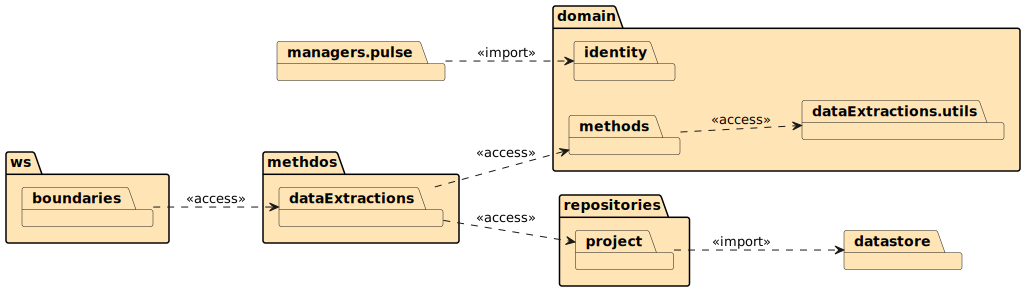
\includegraphics[width =\textwidth, scale=1.0]{Chapter-4/Figures/detection-service.png}
\SourceOrNote{Own authorship (2024)}
\end{figure}
\FloatBarrier

The package \texttt{datastore} is configured with identical database parameters to those defined in \cref{sub-intermediary-packages}.

Package \texttt{ repository.project} has logic to manipulate the database where projects are saved and retrieved for unrefactored and refactored projects. The database configuration, such as the address and ports, is imported from the \texttt{datastore} package.

The package \texttt{methos.dataExtractoins} includes preconfigured interfaces for implementing various code extraction methods. The Abstract Syntax Tree is implemented as the extraction method for the refactoring processes within the RMT. Following the code transformation into an Abstract Syntax Tree (AST), the service accesses the files within the \texttt{domain.mehtos} to perform its designated function.

The package \texttt{managers.pulse} includes the configuration for the service registry, sending requests every minute as proof of life to the intermediary service, and can receive requests. Information, such as the address and port sent from the service, is retrieved from the package \texttt{domain.identity}.

The interfaces for candidates searching and refactoring projects are in the \texttt{domain.methdos} has interfaces to implement and extend the tool refactoring options. As the current methods implement the Abstract Syntax Tree as an extraction method, the \texttt{doamin.dataExtraction.utils} package has methods to facilitate AST manipulation.

To start refactoring, the controllers must receive an HTTP request on the \texttt{ws.boundaries} that distributes the request based on its URL path among the other class functions. 

\subsection{Metrics Service Package Analisys}

The metrics service is divided into six main packages and two main functionalities; as the detection service, the metrics service communicates with the intermediary service for the service registry; the second functionality calculates metrics and quality attributes (calculated with the metrics results). The services have interfaces to increase the available metrics and quality attributes. The \cref{fig-package-metrics} shows the diaram package.

\begin{figure}[ht!]
\SetCaptionWidth{\textwidth}
\caption{Metrics Service Package Diagram}
\label{fig-package-metrics}
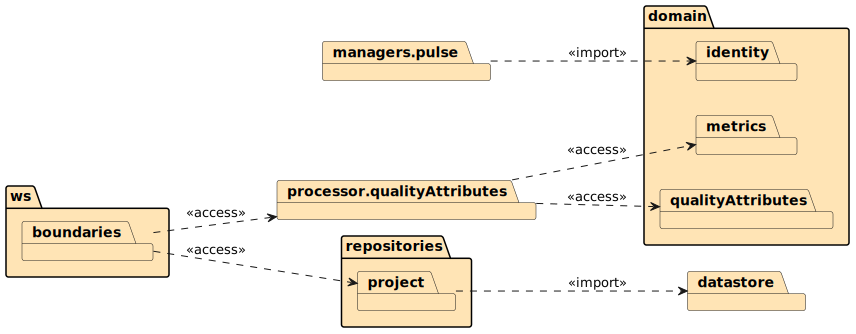
\includegraphics[width =\textwidth, scale=1.0]{Chapter-4/Figures/metrics-service.png}
\SourceOrNote{Own authorship (2024)}
\end{figure}
\FloatBarrier

Consistent with the two preceding services, the \texttt{ datastore} is the repository for all database configuration settings.

To access the unrefactored and refactored projects, the package \texttt{repository.project} has all the logic queries to the database using the information provided by the \texttt{datastore} package.

Correspondingly to the previous service, the package \texttt{managers.pulse} encompasses the comprehensive logic required for registration within the service discovery mechanism. This service adheres stringently to all the specifications delineated in the detection service.

Similarly to the detection service, the \texttt{processor.qualityAttributes} has the interfaces to implement different methods of measuring code metrics and quality attributes. The interfaces' logic and calculations are in the \texttt{domain.metrics} and \texttt{domain.qualityAttribute} packages.

The classes with logic and calculations for generating metrics are in the \texttt{domain.metrics} package; for now, they are hardcoded, implementing the CK module created by \textcite{ck}; however, the interface is designed to integrate additional metrics generation methodologies. In the \texttt{domain.qualityAttributes} package is located in the calculations for quality attributes, such as maintainability, readability, etc.

Consistent with previous services, the \texttt{ws.boundaries} packages serve as the access point for service functionalities. They coordinate computations by interfacing with the database to retrieve project data and invoke methods within the \texttt{processor.qualityAttributes} packages, thereby generating metrics and quality attributes.
 
\section{Improving The Tool With Unit Tests}

Upon comprehending the tool's functionalities, the subsequent step involves verifying the presence of tests. This is essential to commence the refactoring process, as explained by Fowler:

\Citation[english]{\cite[9]{fowler2018refactoring}}{Whenever I do refactoring, the first step is always the same. I need to ensure I have a solid set of tests for that section of code. The tests are essential because even though I will follow refactorings structured to avoid most of the opportunities for introducing bugs, I’m still human and still make mistakes}.

The RMT lacked any form of testing; therefore, according to \textcite{fowler2018refactoring} philosophy, the tool was subjected to unit tests to verify consistent behavior after refactoring. The tests focused on the business logic of the detection service and the quality attribute computations within the metrics service. Testing was bypassed for the intermediary service due to its complete redevelopment.

The tests were designed exclusively for classes with specific logic, excluding interfaces, enumerations (enums), and Plain Old Java Objects (POJOs). This exclusion is justified, as such classes only exhibit the intrinsic behavior provided by the programming language itself without incorporating any additional logic. Consequently, there is no need to test these classes.

\subsection{Designing Test Scenarios for Detection Service}

Tracing the tool's execution path, the initial classes slated for testing are within the \texttt{methods} package, as they are the classes responsible for parsing the code into an Abstract Syntax Tree (AST). After refactoring, the parsing behavior must remain consistent, given that the AST is the foundational structure enabling the tool's capacity to manipulate Java classes to refactor. The \cref{fig-class-detection-methods} illustrates the simplified class diagram for the Methods package.

\begin{figure}[ht!]
\SetCaptionWidth{\textwidth}
\caption{Detection Service Methods Package Simplified Class Diagram}
\label{fig-class-detection-methods}
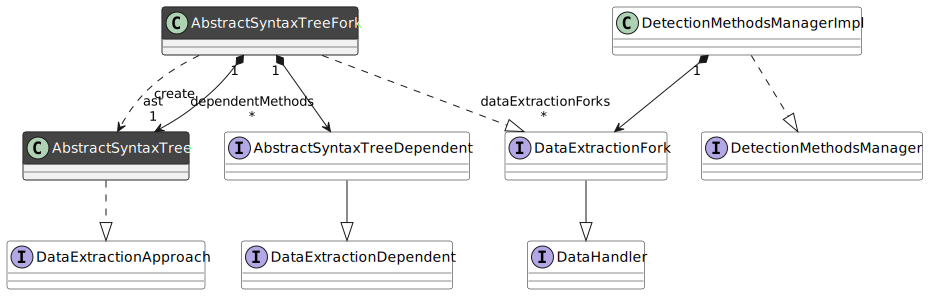
\includegraphics[width =\textwidth, scale=1.0]{Chapter-4/Figures/detection-service-methods.png}
\SourceOrNote{Own authorship (2024)}
\end{figure}
\FloatBarrier

The initial phase of the RMT refactoring process, 'data extraction', involves parsing Java files into an Abstract Syntax Tree (AST), a task performed by the \texttt{AbstractSyntaxTree} class. The class testing methodology involves the accuracy of the parsing process, the generation of an AST object, or the identification of errors as the library \cite{javaparser} executes the process. Therefore, the reliability of this library is assumed, necessitating only the validation of the output. This is achieved by converting a code sample into a string and confirming the equivalence between the AST output, also as a string, and the original input. Error conditions are tested by deliberately invoking the library with incorrect Java code and asserting the results.

The \texttt{AbstractSyntaxTreeFork} class orchestrates the refactoring implemented methods that use the Abstract Syntax Tree (AST) as the parsing mechanism. The refactoring process is divided into two primary stages: invoking methods to identify candidate elements and executing methods to refactor the identified candidate classes. Additionally, the class has logic for database manipulation; this aspect was not subjected to testing due to the substitution of all database communication mechanisms and the database itself, thereby obviating the necessity to preserve any pre-existing behavior. For testing the class, the refactoring techniques had to be mocked (creating an object that simulates the original object's behavior) and assuring the behavior when the methods return an error or success.

The \texttt{DetectionMethodsManagerImpl} was excluded from the testing due to the planned complete reimplementation of the class, which encapsulates the algorithms for project retrieval from the database and the execution of procedures within \texttt{AbstractSyntaxTreeFork}.


The methods executed by \texttt{AbstractSyntaxTree} are situated within the \texttt{methods} package and hold the logic for each implemented refactoring method. The classes are split into two distinct categories: the first category contains classes designed to identify refactoring candidates by detecting specific patterns within Java code that qualify for refactoring; the second category consists of classes intended to execute the refactoring process, thereby effectuating the requisite modifications to the code. The simplified class diagram in \cref{fig-class-detection-domain} represents these classes.

\begin{figure}[ht!]
\SetCaptionWidth{\textwidth}
\caption{Detection Service Domain Package Simplified Class Diagram}
\label{fig-class-detection-domain}
\includegraphics[width =\textwidth, scale=1.0]{Chapter-4/Figures/detection-service-domain.png}
\SourceOrNote{Own authorship (2024)}
\end{figure}
\FloatBarrier

The classes \texttt{WeiEtAl2014Candidate}, \texttt{WeiEtAl2014FactoryCandidate}, \texttt{ZafeirisEtAl2016Candidate}, and \texttt{WeiEtAl2014StrategyCandidate} were excluded from testing, as previously mentioned since Plain Old Java Objects (POJOs) devoid of any business logic were not subjected to testing.

The initial tested class is the \texttt{AstHandler}, serving as an encapsulating wrapper that facilitates direct access to an AST branch. The test cases must ensure that the methods can access the AST objects, such as methods, variables, inner classes, etc. The class also has some methods with limited logic, like assuring that two variables are the same and finding a class's parent, among others. Those functionalities were tested to ensure that they worked as intended and would continue after the refactoring. Some opportunities for improvement were discovered during the development of test cases, which are addressed in \cref{results}. 

Agrupar as classes de encotrar candidados do wei, e explicar como testar

\subsection{Designing Test Scenarios for Metrics Service}

\section{Refatoracao}

\subsection{Refactoring And Metrics Manager Service}

\subsection{Detection And Refactoring Service}

\subsection{Metrics Calculation Service}

\section{Teste da ferramenta}